\chapter{Introducción}
\label{cap:introduccion}

\chapterquote{En tiempos de engaño universal, decir la verdad se convierte en un acto revolucionario.}{George Orwell}

\section{Motivación}
A lo largo de los años, los videojuegos han experimentado una notable evolución, transformándose en elementos más complejos. En paralelo, los enemigos han tenido la misma evolución. En el contexto específico de los videojuegos de plataformas en dos dimensiones, los enemigos son más que una simple oposición del jugador, son la clave para mostrar la esencia del juego. Diseñar enemigos, especialmente en el tipo de videojuegos mencionados, es una tarea cada vez más compleja. No se limita a darles cierta apariencia sino que tienen que tener unos comportamientos y características únicas. Como consecuencia, provocamos que la persona encargada de realizar esta tarea tenga que tener ciertos conocimientos multidisciplinares (arte, diseño, programación ...). 
En los últimos años han surgido herramientas destinadas a simplificar significativamente el flujo de trabajo de los diseñadores. No obstante, una proporción limitada de estas se enfoca específicamente a este espacio de trabajo. El propósito de estas herramientas reside en facilitar la labor de los diseñadores, permitiéndoles, incluso sin dominio de la programación, la capacidad de generar enemigos con funcionalidades completas.

\section{Objetivos}
Este trabajo tiene como objetivo principal el diseño y desarrollo de un framework para el motor de videojuegos \textit{Unity} que simplifique y agilice el proceso de creación de enemigos en juegos plataformas 2D. Este framework define una estructura modular de componentes y comportamientos basada en el análisis de enemigos comunes en este tipo de juegos, con el fin de separar completamente los roles de programación y diseño. De este modo, se facilita que personas sin conocimiento de programación puedan desempeñar el rol de diseñador de enemigos.\\

Como ejemplificación práctica del framework, se ha desarrollado una herramienta funcional en Unity que permite implementar y utilizar estos componentes de manera visual e intuitiva. La herramienta incluye un catálogo de comportamientos fácil de manejar para cualquier persona, así como un manual de usuario que explica claramente cada componente, su instalación y ejemplos de uso.\\

Para llevar a cabo este desarrollo, se ha seguido un plan de trabajo estructurado que abarca desde el estudio del entorno y la revisión de enemigos existentes, hasta la implementación de la herramienta, su validación con usuarios y el análisis de los resultados obtenidos.\\

\section{Plan de trabajo}
Para llevar a cabo este trabajo, se ha seguido la metodología ágil Scrum. Esta metodología, permite crear un flujo de trabajo enfocado en la iteración y continua mejora, asegurando un avance en el desarrollo eficiente y posibles adaptaciones frente a problemas detectados durante el proceso. 
El trabajo se dividirá en cuatro bloques: investigación y planificación, desarrollo de la memoria, desarrollo de la herramienta y pruebas con usuarios.
Cada bloque a su vez se dividirá en subsecciones explicadas a continuación.
\begin{itemize}
   \item  Investigación y planificación:
	\begin{itemize}
	    \item  Estudio del problema: En esta primera fase se realizará un estudio del estado del arte, centrado en el papel de los enemigos en los videojuegos, su importancia en la jugabilidad y las diferentes técnicas utilizadas para su diseño y comportamiento.
	    \item Selección y estudio de herramientas: Esta fase implicará un análisis comparativo de distintas técnicas y motores de videojuegos evaluando sus ventajas y desventajas, así como un estudio de su funcionamiento y  arquitecturas.
	    \item Estudio de comportamientos de enemigos: Este estudio nos permitirá tener una base solida para el diseño de la herramienta por medio de la identificación de similitudes en los comportamientos de distintos enemigos. 
	\end{itemize}
   \item Desarrollo de la herramienta: 
	\begin{itemize}
	    \item Diseño: En esta etapa, se definirá la arquitectura de la herramienta propuesta describiendo las técnicas empleadas, esquemas de funcionamiento y organización de elementos principales.
	    \item  Implementación de funcionalidades principales: En esta etapa se implementarán las funcionalidades principales de los movimientos básicos incluyendo la integración con sensores y actuadores permitiendo la interacción entre ellos.
	    \item Implementación de ayuda visual: Se desarrollarán ayudas visuales destinadas a servir como referencias para los diseñadores, incluyendo elementos gráficos que faciliten la comprensión de los comportamientos. 
	    \item Pruebas y depuración: Se llevará a cabo un proceso iterativo de pruebas que aseguren la funcionalidad de la herramienta, corrigiendo los errores detectados durante su implementación.
	\end{itemize}
   \item Pruebas con usuarios:
	\begin{itemize}
	    \item Se harán pruebas con usuarios que no hayan probado la herramienta antes, siguiendo un plan de pruebas especificado en el apartado \hyperref[cap:evaluacionConUsuarios]{evaluación con usuarios}. Las pruebas estarán centradas en detectar posibles errores en las funcionalidades principales, validar la funcionalidad y evaluar la usabilidad y claridad.
	\end{itemize}
   \item Desarrollo de la memoria: 
	\begin{itemize}
	    \item  Redacción inicial: Es esta fase del trabajo se procederá a la redacción inicial de los contenidos cubriendo todos los puntos especificados en el índice.
	    \item Revisión y corrección: Una vez completada la redacción inicial, se realizarán las correcciones necesarias tras revisar exhaustivamente el documento.
	    \item Conclusiones y trabajo futuro: Tras finalizar los desarrollos y las pruebas de usuario, se redactarán las conclusiones obtenidas en base a los resultados y se detallarán los posibles pasos a seguir en un futuro.
	\end{itemize}
\begin{figure}[h!]
	\centering
	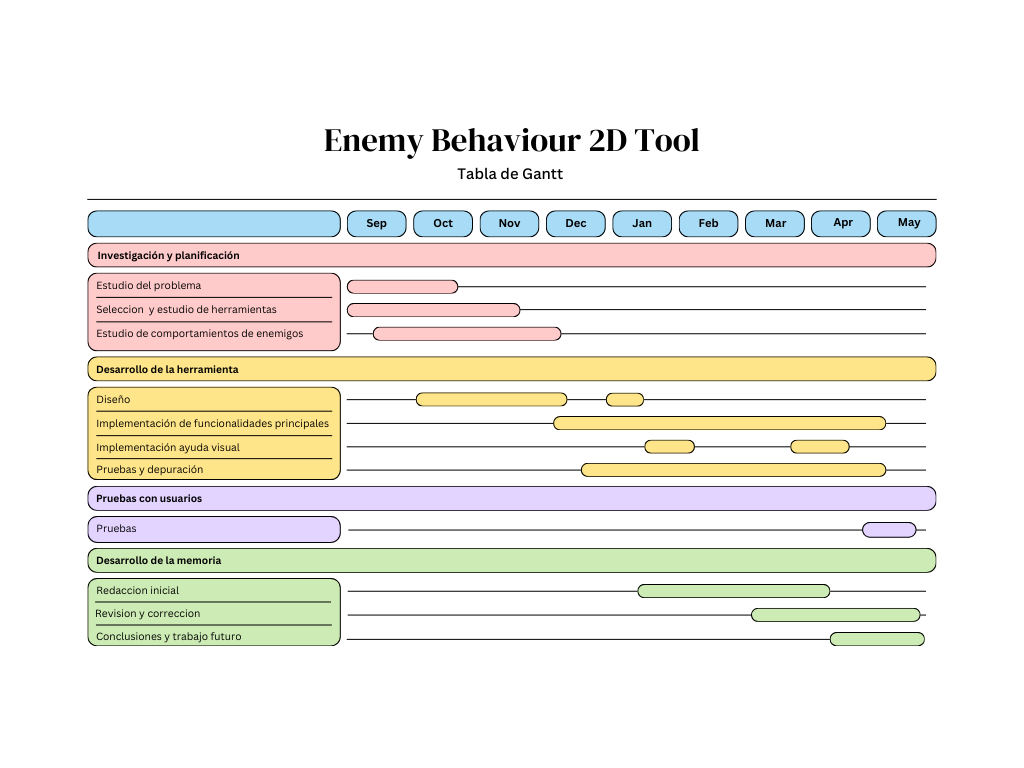
\includegraphics[height=12cm]{Imagenes/GanttChart}
	\caption{Diagrama de planificación del desarrollo de la herramienta Enemy Behaviour 2D}
	\label{fig:GanttEnemyBehaviour2D}
\end{figure}

\end{itemize}
